\section{緒言}

\subsection{研究背景}
一般的に,流体はせん断応力がひずみ速度に比例するニュートン流体と,せん断応力がひずみ速度が非線形となる非ニュートン流体に分類することができる.粘性応力とひずみ速度の比例係数として用いられる粘度について考えると,ニュートン流体ではせん断速度に関わらず一定となっている.一方で非ニュートン流体において,粘度はせん断速度によって変化する.

Fig.\ref{fig:1-fluid-curve}に示す通り,非ニュートン流体はDilatant fluid, Pseudoplastic, Bingham plastic, Viscoplastic が挙げられている.これら非ニュートン流体の粘度を示す理論として,Power-law model (Ostwald-De Waele model), Cross model,Carreau viscosity equationやHerschel-Bulkley modelなどを挙げることができる\cite{ref:1}.Power-law model はせん断速度の限られた範囲内にて適応することができる.理論式中の指数によってニュートン流体,shear-thinning流体と,shear-thickening流体に分類することができる.これらのせん断速度と粘度の関係性はFig.\ref{fig:2-Newton-fluid}に示す通りである.これら2種類の流体のうち,shear-thinning流体は,せん断速度$\dot{\gamma}$が高くなるほど粘度$\mu$が低くなる性質を有している.この流体は擬塑性流体とも呼ばれている.

Cross modelはshear-thinning性が構造的に引き起こされるといった仮説において導き出された理論である.これは広いせん断速度において適用することができる.また,Carreau viscosity equationはCross modelをpower-law領域においてより適合するよう修正したものとなっている.Herschel-Bulkley modelはBingham plasticやViscoplasticといった静止状態の流体においてせん断応力が存在する流体を示す理論となっている\cite{ref:1}.

擬塑性流体とは,液状で巨大な分子が存在する流体や固体粒子が懸濁状で液体に存在する流体のことである.擬塑性流体の一般的な例として,砂や砂利など粒状の物質と水が混合する,泥流や雪崩といった自然現象を挙げることができる.また,産業分野において,擬塑性流体を混合や輸送行うことがある.効率よく輸送や混合を行うためには,擬塑性流体中の分散体周囲の粘度分布,流動構造から擬塑性が分散体に及ぼす影響を明らかにする必要がある.

例えばOhtae {\it et al.} \cite{ref:2}は非弾性擬塑性流体中において液滴の上昇運動に対し,数値計算,実験から液滴周りのせん断速度による粘度低下があたえる影響を明らかにした.また,液滴周りの粘度分布を数値計算で求め,局所的な粘度低下は液滴の形状に大きく依存することが報告されている\cite{ref:3}.また,Zhang {\it et al.} \cite{ref:4}は非弾性擬塑性流体中における単一気泡の上昇運動に対し,数値計算,実験から,気泡周囲のせん断速度,粘度,速度場を明らかにした.Iwata {\it et al.}\cite{ref:5}は擬塑性流体中における気泡の体積を周期的に増加・減少させ上昇速度を増加させた.さらに,Fig.\ref{fig:3-bubble}に示すように気泡が膨張時には球形であっても収縮時には気泡下部がとがったカスブ形状に変化されることも報告された.これらは気泡近傍の複雑流れと流体の弾性が影響していると考えられている.超音波振動の影響による擬塑性流体における抵抗低下に関してvan den Wildenberg {\it et al.}\cite{ref:6}による研究があげられる.本研究では,粒子の上部を水で満たし容器ごと振動させ,水と混合することで擬塑性流体を発生させた.その擬塑性流体中に球を落下させ,その落下球の速度や位置に関しての計測を行った.その結果をFig.\ref{fig:4-sinking}に示す.Fig.\ref{fig:4-sinking}(a1)において,$\Gamma$は振動強度である.振動によって落下球表面におけるせん断応力が減少したため振動強度を強くするとより深くまで沈降すると報告された.

本研究では,擬塑性流体中を落下する鋼球へ超音波を照射し,落下球の近傍における流体の粘度を局所的に低下させることで,球の落下運動の高速化をはかった.鋼球の落下速度に対しての超音波照射による影響を調べた.

\begin{center}
    \begin{figure}[h]
        \centering
        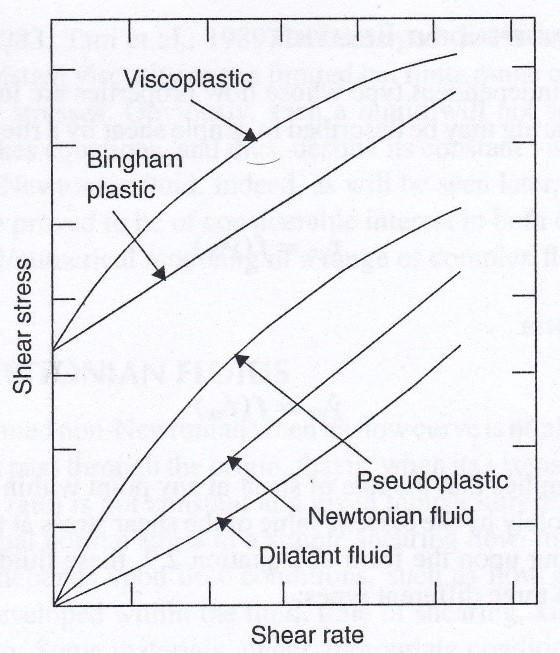
\includegraphics[width=7.0cm,clip]{1-Background/1-fluid-curve.jpg}
        \caption{Qualitative flow curves for different types of non-Newtonian fluids\cite{ref:1}.}
        \label{fig:1-fluid-curve}
        \centering
        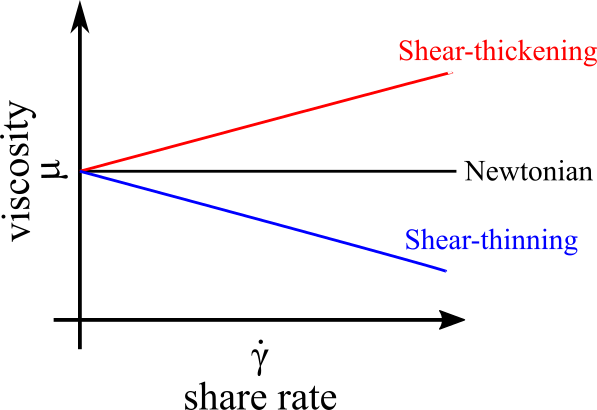
\includegraphics[width=7.0cm,clip]{1-Background/2-Newton-fluid.png}
        \caption{Classifications of non-Newtonian fluid.}
        \label{fig:2-Newton-fluid}
    \end{figure}

    \newpage

    \begin{figure}[h]
        \centering
        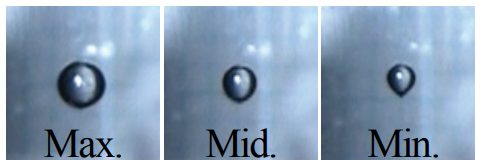
\includegraphics[width=10.0cm,clip]{1-Background/3-bubble.png}
        \caption{Periodic change in shape of bubble under cyclic pressure change\cite{ref:5}.}
        \label{fig:3-bubble}
        \centering
        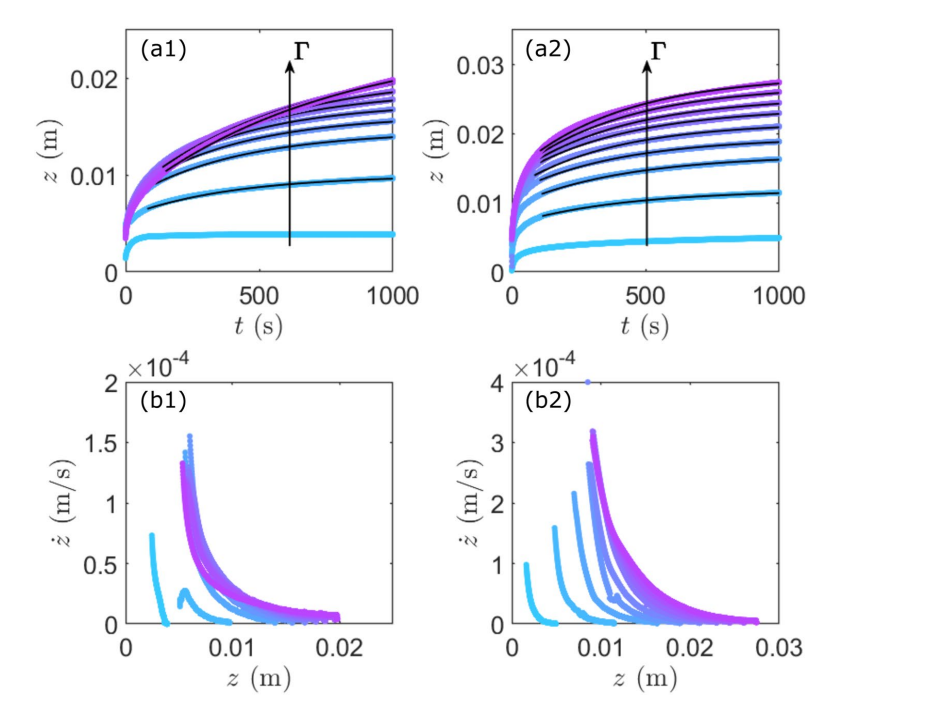
\includegraphics[width=10.0cm,clip]{1-Background/4-sinking.png}
        \caption{Sinking dynamics for different intruder-sizes and for different vibration intensities $\Gamma$. (a1) Depth versus time for an intruder with R=4mm and (a2) for an intruder with R=7mm. (b1) Instantaneous velocity versus sinking depth obtained from (a1) and (b2) from (a2). The black lines correspond to the solutions fitted in the quasi-steady regime\cite{ref:6}.}
        \label{fig:4-sinking}
    \end{figure}
\end{center}

\subsection{研究目的}
擬塑性流体は強いせん断力により粘度が低下していくため,境界層が物体周囲に形成された際に,物体の周囲流体の粘性応力が小さくなり,物体に働く粘性抵抗が低減することから,物体の運動を促進することが可能となる.物体周囲に境界層が形成される要因として,音場により物体周囲に形成される音響境界層がある\cite{ref:7}.この音響境界層内部の粘度を低下させることで落下する球に作用する粘性抵抗が小さくなり,落下速度が増加することが先行研究\cite{ref:8}にて示唆されている.

擬塑性流体の一部領域のみに超音波による強い圧力場が形成された系において落下球の速度を測定し,音響境界層が落下球の速度に及ぼす影響を明らかにすることを目的とする.
本機能デザイン研究において,十分に妥当性が検証された先行研究における実験計測法を習得することを目的とする.また,実験方法の違いによる影響に関して,観測することも一つの目的ともする.
